\documentclass[11pt,a4paper,twoside]{book}

\usepackage[utf8]{inputenc}
\usepackage{amsmath}
\usepackage{amssymb}
\usepackage{amsfonts}
\usepackage{theorem}
\usepackage{fancyheadings}
\usepackage{graphicx}
\usepackage{hyperref}
\usepackage{listings}
\usepackage{makeidx}
\usepackage[all]{xypic}

%%% Settings for listings
\lstset{basicstyle=\ttfamily,xleftmargin=\parindent}

%\newenvironment{proof}{\medskip\noindent\emph{Proof.}}{\hfill$\Box$\medskip}

\newcommand{\defemph}[1]{\emph{\textbf{#1}}}

%%% Blackboard bold letters
\newcommand{\NN}{\mathbb{N}}
\newcommand{\NNx}{{\NN^{+}}}
\newcommand{\ZZ}{\mathbb{Z}}
\newcommand{\QQ}{\mathbb{Q}}
\newcommand{\RR}{\mathbb{R}}
\newcommand{\CC}{\mathbb{C}}

%%% PCAs
\renewcommand{\AA}{\mathbb{A}}
\newcommand{\subAA}{\mathbb{A}'}
\newcommand{\EE}{{\mathbb{E}}}
\newcommand{\subEE}{{\mathbb{E}'}}
\newcommand{\FF}{{\mathbb{F}}}
\newcommand{\subFF}{{\mathbb{F}'}}
\newcommand{\GG}{{\mathbb{G}}}
\newcommand{\subGG}{{\mathbb{G}'}}

\newcommand{\klone}{\mathbb{K}_1}
\newcommand{\UU}{\mathbb{U}}

\newcommand{\CL}{\mathbb{CL}}

%%% Applicative morphisms
\newcommand{\ff}[1]{\widehat{#1}}  % functor induced by an applicative morphism



%%% quantifiers
\newcommand{\all}[1]{\forall #1 .\,}
\newcommand{\some}[1]{\exists #1 .\,}
\newcommand{\lam}[2]{\lambda #1 .\,#2}
\newcommand{\of}{{:}}

%% Grammar
\newcommand{\bnfis}{\mathbin{{:}{:}{=}}}
\newcommand{\bnfor}{\mid}

%%% Substitution
\newcommand{\subst}[2]{#1[#2]}

%%% Arrows
\newcommand{\subto}{{\shortrightarrow}} % for substitution
\newcommand{\oneto}{\mapsto}
\newcommand{\manyto}{\oneto^{*}}
\newcommand{\multito}{\rightrightarrows}
\newcommand{\parto}{\mathbin{\rightharpoonup}}
\newcommand{\epito}{\twoheadrightarrow}
\newcommand{\into}{\hookrightarrow}
\newcommand{\monoto}{\rightarrowtail}
\newcommand{\natto}{\Rightarrow} % natural transformation

\newcommand{\curry}[1]{\hat{#1}}
\newcommand{\uncurry}[1]{\check{#1}}

%%% Sets
\newcommand{\set}[1]{\{#1\}}
\newcommand{\such}{\mid}
\newcommand{\pow}[1]{\mathcal{P}(#1)}

\newcommand{\im}[1]{\mathrm{im}(#1)}

\newcommand{\tbigcup}{\bigcup\nolimits}
\newcommand{\tbigcap}{\bigcap\nolimits}

\newcommand{\dsum}{\Sigma}
\newcommand{\dprod}{\Pi}

\newcommand{\zero}{\mathsf{0}}
\newcommand{\one}{\mathsf{1}}
\newcommand{\two}{\mathsf{2}}

\newcommand{\NNNN}{\NN^{\NN}}
\newcommand{\Sierpinski}{\mathbb{S}}
\newcommand{\Baire}{\mathbb{B}}
\newcommand{\Cantor}{\two^{\NN}}
\newcommand{\Scott}{\mathbb{P}}

%%% Topology
\newcommand{\topol}[1]{\mathcal{O}(#1)}

%%% Functions
\newcommand{\id}[1][]{\mathrm{id}_{#1}}

\newcommand{\dom}[1]{\mathsf{dom}(#1)}
\newcommand{\invim}[1]{#1^{*}}
\newcommand{\inv}[1]{{#1}^{-1}}

\newcommand{\defined}[1]{#1{\downarrow}}
\newcommand{\divergent}[1]{#1{\uparrow}}
\newcommand{\place}{{-}}

\newcommand{\restrict}[2]{#1{\restriction}_{#2}}

%%% Pairing
\newcommand{\pair}[1]{\langle #1 \rangle}
\newcommand{\xfst}{\mathtt{fst}}
\newcommand{\fst}[1]{\xfst,#1}
\newcommand{\xsnd}{\mathtt{snd}}
\newcommand{\snd}[1]{\xsnd,#1}

%%% Coding
\newcommand{\code}[1]{\ulcorner #1 \urcorner}

%%% Standard enumerations
\newcommand{\enumstage}[2]{#1{\mid}_{#2}}

\newcommand{\xpr}{\text{\boldmath{$\varphi$}}}
\newcommand{\pr}[2]{\xpr_{#1}(#2)}
\newcommand{\prm}[3]{\xpr^{(#1)}_{#2}(#3)}

\newcommand{\iitm}[1]{\text{\boldmath{$\psi$}}_{#1}}

\newcommand{\xfpr}{\text{\boldmath{$\eta$}}}
\newcommand{\fpr}[2]{\xfpr_{#1}(#2)}
\newcommand{\fprm}[3]{\xfpr^{(#1)}_{#2}(#3)}

\newcommand{\cons}[2]{#1 {:}{:} #2}
\newcommand{\append}[2]{#1 \mathbin{{+}\!\!{+}} #2}
\newcommand{\basicBB}[1]{#1{{+}\!\!{+}}\Baire}
\newcommand{\seq}[1]{[#1]}
\newcommand{\seg}[2]{\overline{#1}(#2)}

%%% Lambda calculus
\newcommand{\unit}{\mathtt{unit}}
\newcommand{\ttunit}{{\star}}
\newcommand{\ttfst}[1]{\mathtt{fst}\,#1}
\newcommand{\ttsnd}[1]{\mathtt{snd}\,#1}
\newcommand{\FV}[1]{\mathsf{FV}(#1)}
\newcommand{\ttnat}{\mathtt{nat}}
\newcommand{\ttbool}{\mathtt{bool}}

%% Denotational semantics
\newcommand{\sem}[1]{[\![#1]\!]}

%% Logic
\newcommand{\ctx}{\mid}

\newcommand{\lthen}{\Rightarrow}
\newcommand{\liff}{\Leftrightarrow}


% Axiom
\newcommand{\axiom}[1]{\dfrac{}{#1}}

% Axiom with a side condition
\newcommand{\axiomd}[2]{\dfrac{}{#1} \; #2}

% Inference rule
\newcommand{\infer}[2]{\begin{gathered}\dfrac{#1}{#2}\end{gathered}}
\newcommand{\inferr}[3]{\begin{gathered}\dfrac{#1\quad #2}{#3}\end{gathered}}
\newcommand{\inferrr}[4]{\begin{gathered}\dfrac{#1\quad #2 \quad #3}{#4}\end{gathered}}

\newcommand{\sep}{\qquad}
\newcommand{\fromassumption}[2]{
  \begin{gathered}[b]
    {\displaystyle #1} \\
    \vdots \\
    {#2}
  \end{gathered}}

% Inference rule with a side condition
\newcommand{\inferd}[3]{\begin{gathered}\dfrac{#1}{#2} \; #3\end{gathered}}

%%% Domain theory
\newcommand{\upper}[1]{{\uparrow}#1}
\newcommand{\wayb}{\ll}

%%%% PCAs
\renewcommand{\AA}{\mathbb{A}}
%\newcommand{\compAA}{\comp{\AA}}

\newcommand{\pcalam}[1]{\langle #1 \rangle\,}
\newcommand{\annot}[2]{#1^{#2}}
\newcommand{\tpcalam}[2]{\langle \annot{#1}{#2} \rangle\,}
\newcommand{\kleq}{\simeq}
\newcommand{\klgeq}{\succeq}
\newcommand{\numeral}[1]{\overline{#1}}
\newcommand{\JJ}{\mathbb{J}}

\newcommand{\pcacomb}[1]{\mathtt{#1}}

%\newcommand{\pcato}{\stackrel{\scriptscriptstyle\mathsf{PCA}}{\longrightarrow}}
\newcommand{\pcato}{\xrightarrow{\scriptscriptstyle\mathsf{pca}}{}}

\newcommand{\combK}{\pcacomb{K}}
\newcommand{\combS}{\pcacomb{S}}
\newcommand{\combI}{\pcacomb{I}}

\newcommand{\combY}{\pcacomb{Y}}
\newcommand{\combZ}{\pcacomb{Z}}
\newcommand{\combW}{\pcacomb{W}}
\newcommand{\combFix}{\pcacomb{fix}}

\newcommand{\combPair}{\pcacomb{pair}}
\newcommand{\combFst}{\pcacomb{fst}}
\newcommand{\combSnd}{\pcacomb{snd}}

\newcommand{\combLeft}{\pcacomb{left}}
\newcommand{\combRight}{\pcacomb{right}}
\newcommand{\combCase}{\pcacomb{case}}

\newcommand{\combSucc}{\pcacomb{succ}}
\newcommand{\combPred}{\pcacomb{pred}}

\newcommand{\combRec}{\pcacomb{rec}}
\newcommand{\combMin}{\pcacomb{min}}

\newcommand{\combIf}{\pcacomb{if}}
\newcommand{\combTrue}{\pcacomb{true}}
\newcommand{\combFalse}{\pcacomb{false}}
\newcommand{\combIsZero}{\pcacomb{iszero}}
\newcommand{\cond}[3]{\mathtt{if}\,#1\,\mathtt{then}\,#2\,\mathtt{else}\,#3}

\newcommand{\case}[5]{\mathtt{case}\,#1\,\mathtt{of}\,#2 \mapsto #3 \mid #4 \mapsto #5}
\newcommand{\xcase}[5]{\begin{aligned}[t]\mathtt{case}\,&#1\;\mathtt{of}\\&#2 \mapsto #3 \\&#4 \mapsto #5\end{aligned}}


% PCF
\newcommand{\PCF}{\mathsf{PCF}}
\newcommand{\PCFinf}{\mathsf{PCF}^\infty}


% Realizability
\newcommand{\comp}[1]{#1_{\#}}
\newcommand{\rz}[1][]{\Vdash_{#1}}
\newcommand{\Ex}[1][]{\mathsf{E}}
\newcommand{\per}{\approx}

\newcommand{\typ}[2]{#1_{#2}}
\newcommand{\Atyp}[1]{\typ{\AA}{#1}}
\newcommand{\xAtyp}[1]{\typ{\AA}{|#1|}}
\newcommand{\subAtyp}[1]{\typ{\subAA}{#1}}

\newcommand{\effsym}{\#}
\newcommand{\eff}[1]{\effsym #1}

\newcommand{\R}[1]{\mathtt{#1}} % realizer
\renewcommand{\S}[1]{|#1|} % underlying set 
\newcommand{\T}[1]{\|#1\|} % underlying type
\newcommand{\xasm}[1]{(\S{#1|}, \T{#1}, {\rz[#1]})}
%\newcommand{\asm}[1]{#1}

\newcommand{\rep}[1]{\mathbf{#1}}
\newcommand{\xrep}[1]{(#1, \delta_{#1})}

% Categories

\newcommand{\cat}[1]{\mathcal{#1}}
\newcommand{\Hom}[1]{\mathsf{Hom}(#1)}

\newcommand{\Sub}[1]{\mathsf{Sub}(#1)}
\newcommand{\Mono}[1]{\mathsf{Mono}(#1)}
\newcommand{\Pred}[1]{\mathsf{Pred}(#1)}

%\newcommand{\subcat}[1]{\mathsf{Subset}(#1)}

\newcommand{\Set}{\mathsf{Set}}
\newcommand{\Asm}[1]{\mathsf{Asm}(#1)}
\newcommand{\AsmA}{\Asm{\AA,\subAA}}

\newcommand{\Mod}[1]{\mathsf{Mod}(#1)}
\newcommand{\ModA}{\Mod{\AA,\subAA}}

\newcommand{\Rep}[1]{\mathsf{Rep}(#1)}
\newcommand{\Per}[1]{\mathsf{Per}(#1)}
\newcommand{\Er}[1]{\mathsf{Er}(#1)}

\newcommand{\wTop}{\mathsf{\omega Top}}
\newcommand{\compTop}{\comp{\wTop}}
\newcommand{\Equ}{\mathsf{Equ}}

\newcommand{\CanProj}[1]{\mathsf{Proj}(#1)}

% Adjunctions

% Adjunction as a two-way rule
\newcommand{\adjunction}[2]{%
  \begin{tabular}{c}
    $#1$ \\
    \noalign{
      \vskip 2pt      
      \hrule
      \vskip 1pt      
      \hrule
      \vskip 2pt      
      }
    $#2$
  \end{tabular}
  }

\newcommand{\adjunctionx}[3]{%
  \begin{tabular}{c}
    $#1$ \\
    \noalign{
      \vskip 2pt      
      \hrule
      \vskip 1pt
      \hrule
      \vskip 2pt      
      }
    $#2$ \\
    \noalign{
      \vskip 2pt      
      \hrule
      \vskip 1pt
      \hrule
      \vskip 2pt      
      }
    $#3$
  \end{tabular}
  }

\newcommand{\adjrule}{\noalign{\vskip 2pt \hrule \vskip 1pt \hrule \vskip 2pt}}

\newcommand{\longadjunction}[1]{
\begin{tabular}{>{$}c<{$}}
#1
\end{tabular}
}



%%% Local Variables: 
%%% mode: latex
%%% TeX-master: "notes-on-realizability"
%%% End: 


%%% Index
\makeindex

%% A4 stran = 210mm x 297mm
%% sirino besedila nastavimo na 170mm, visino na 247mm

\setlength{\textwidth}{15cm}
\setlength{\textheight}{224mm}

\setlength{\topmargin}{0cm}
\setlength{\evensidemargin}{0cm}
\setlength{\oddsidemargin}{\paperwidth}

\addtolength{\oddsidemargin}{-\textwidth}
\addtolength{\oddsidemargin}{-2in}

\addtolength{\headwidth}{\marginparsep}
\addtolength{\headwidth}{\marginparwidth}

%%%%%%%%%%%%%%%%%%%%%%%%%%%%%%%%%%%%%%%%%%%%%%%%%%%%%%%%%%%%%%%%%%%%%%
%% For Draft versions uncomment this:
\newcommand{\draftnote}{{\textsc{[DRAFT: \today]}}}
%% For official non-draft version, uncomment this:
%\newcommand{\draftnote}{}

\pagestyle{fancyplain}

\setlength{\headrulewidth}{0.2pt}
\addtolength{\headheight}{2pt}

\renewcommand{\chaptermark}[1]{\markboth{#1}{}}
\renewcommand{\sectionmark}[1]{\markright{\thesection\ #1}}
\lhead[\fancyplain{}{{\thepage}}]{\fancyplain{}{{\rightmark}}}
\rhead[\fancyplain{}{{\leftmark}}]{\fancyplain{}{\thepage}}
\cfoot{}
\lfoot[]{\fancyplain{{\scriptsize\draftnote}}{{\scriptsize\draftnote}}}
\rfoot[\fancyplain{{\scriptsize\draftnote}}{{\scriptsize\draftnote}}]{}

\newcommand{\clearemptydoublepage}{\newpage{\pagestyle{empty}\cleardoublepage}}


\begin{document}

\title{
  The Realizability Approach to\\
  Computable Analysis and Topology\\
  (Lecture notes)
}

\author{Andrej Bauer}

\maketitle

%%%%%%%%%%%%%%%%%%%%%%%%%%%%%%%%%%%%%%%%%%%%%%%%%%%%%%%%%%%%%%%%%%%%%%
%%%% Preface

\chapter*{Preface}

I sometimes think it is unfortunate that the modern mathematics of
20${}^{\text{th}}$ century came before modern computers. Perhaps it is
true that computers would have never been invented without Hilbert's
putting a decision problem on his list, G\"odel's unbelievable
exercise in programming with numbers, the discovery of
$\lambda$-calculus, recursive functions, and Turing's machines, but by
the time computers ruled the world, generations of mathematicians had
been educated with little regard to questions about computability of
mathematical structures. They were told their world was a paradise and
were encouraged to take pride in the uselessness of their activity.
Today classical mathematics is taken for granted by the vast majority
of mathematicians, despite overwhelming evidence that we have entered
an era of computable---and therefore non-classical---mathematics.

How does a classically trained mathematician approach computability of
real numbers and other structures in mathematical analysis? Given the
unshakable edifice of classical mathematics that he knows, it is only
natural for him to ``bolt on computability as an afterthought'', as a
friend of mine once put it. Indeed, this is how computable mathematics
is practiced by most experts, and this is also the way in which we
approach the subject. However, after introducing the basic models of
computability and the theory of representations, we take a general
look at the setup from the viewpoint of realizability theory, through
which the connection with constructive mathematics emerges. We develop
the tools necessary to tackle the subject in an abstract and
conceptual way. It turns out that computable mathematics is just
ordinary, albeit constructive, mathematics developed in mathematical
universes that have computability built in from their conception. In
the final chapter we put on programmer's hat and actually implement
some of the computable structures in a real-world programming
language.

These lecture notes were prepared for a graduate course at the Faculty
of Mathematics and Physics, University of Ljubljana, Slovenia. I have
included more material than I could hope to cover in 15 lectures,
90~minutes each. I am aware that proper understanding of the subject
requires background knowledge in computability theory, analysis,
topology, logic, category theory, and programming. Therefore, the
first exercise for the vigilant students is to look up the meaning of
the Japanese word \emph{shugyo}.


\bigskip

\begin{flushright}
Andrej Bauer\\
Ljubljana, January 2009
\end{flushright}


%%%%%%%%%%%%%%%%%%%%%%%%%%%%%%%%%%%%%%%%%%%%%%%%%%%%%%%%%%%%%%%%%%%%%%
%%%% Table of contents

\clearemptydoublepage

\markboth{}{Contents}
{
\renewcommand{\markboth}[2]{}
\tableofcontents
}

%%%%%%%%%%%%%%%%%%%%%%%%%%%%%%%%%%%%%%%%%%%%%%%%%%%%%%%%%%%%%%%%%%%%%%
%%%% Chapters

\chapter{Introduction}
\label{chap:introduction}

\section{Background material}
\label{sec:background-material}

In this section we overview a selection of concepts which we need
later on. We also fix notation and a number of definitions. At the
momement the sections are not listed in any particular order.

\subsubsection*{Free and bound variables}

Occurrences of variables in an expression may be \defemph{free} or
\defemph{bound}. Variables are bound when they are used to indicate the
range over which an operator acts. For example, in expressions
%
\begin{equation*}
  \xall{x}{\RR}{x^2 + y \geq 0},
  \qquad\qquad
  \sum_{k = 0}^n \frac{1}{k^2},
  \qquad\qquad
  \int_a^b f(t) \, dt,
\end{equation*}
%
the variables $x$, $k$, and $t$ are bound by the operators $\forall$,
$\sum$, and $\int$, respectively. The remaining variables are free. It
is really the \defemph{occurrence} of a variable that is bound or free,
not the variable itself. In
%
\begin{equation*}
  P(x) \lor \xusome{x}{\lnot Q(x)}
\end{equation*}
%
the left-most occurence of $x$ is free whereas the other two are bound
by~$\exists$.

\subsubsection*{Functions}

The set of all functions from $A$ to $B$ is denoted by $B^A$ as well as $A \to B$. The arrow associates to the right,
$A \to B \to C$ is $A \to (B \to C)$. We write $f : A \to B$ instead of $f \in A \to B$. If $f : A \to B$ and $x \in A$, the application $f(x)$ is also written as $f\, x$. We often work with \defemph{curried} functions which take several
arguments in succession, i.e., if $f : A \to B \to C$ then $f$ takes $x \in A$, and $y \in B$ to produce an element
$f(x)(y)$ in $C$, also written $f\, x\, y$.


\subsubsection*{Partial functions}

A \defemph{partial} function\sidenote{In the literature on Type Two
  Effectivity the common notation is $f \mathbin{{:}{\subseteq}} A \to
  B$.} $f: A \parto B$ is a function that is defined on a subset
$\dom{f} \subseteq A$, called the \emph{domain} of~$f$. Sometimes
there is confusion between the domain~$\dom{f}$ and the set~$A$, which
is also called the domain. In such cases we call $\dom{f}$ the
\defemph{support} of~$f$. If $f: A \parto B$ is a partial function and $x
\in A$, we write $\defined{f\, x}$ to indicate that $f x$ is defined.
For an expression~$e$, we also write $\defined{e}$ to indicate
that~$e$ and all of its subexpressions are defined. The
symbol~$\downarrow$ is sometimes inserted into larger expressions, for
example, $\defined{f\, x} = y$ means that $f x$ is defined and is
equal to~$y$. If $e_1$ and $e_2$ are two expressions whose values are
possibly undefined, we write $e_1 \kleq e_2$ to indicate that either
$e_1$ and $e_2$ are both undefined, or they are both defined and
equal. The notation $e_1 \klgeq e_2$ means that if $e_1$ is defined
then $e_2$ is defined and they are equal. Thus we have
%
\begin{equation*}
  e_1 \kleq e_2 \iff e_1 \klgeq e_2 \land e_2 \klgeq e_1.
\end{equation*}

A partial map $f: X \parto Y$ between topological spaces~$X$ and~$Y$
is said to be \defemph{continuous} when it is continuous as a total map
$f: \dom{f} \to Y$, where the domain of definition $\dom{f} \subseteq
X$ is equipped with the subspace topology.



\subsubsection*{Primitive recursive and recursive function}

The \defemph{primitive recursive function} are those function $\NN^k \to
\NN$ that are built inductively from the following functions and operations:
%
\begin{enumerate}
\item constant functions $f(n_1, \ldots, n_k) = c$, where $c \in \NN$,
\item projections $p_i(n_1, \ldots, n_k) = n_i$, where $1 \leq i \leq k$,
\item the successor function $s(n) = n + 1$,
\item composition of functions,
\item primitive recursion: given primitive recursive $f : \NN^k \to
  \NN$ and $g : \NN^{k+2} \to \NN$, the function $h : \NN^{k+1} \to
  \NN$ defined by
  %
  \begin{align*}
    h(0, n_1, \ldots, n_k) &= f(n_1, \ldots, n_k), \\
    h(n+1, n_1, \ldots, n_k) &= g(h(n, n_1, \ldots, n_k), n, n_1,
    \ldots, n_k)    
  \end{align*}
  %
  is primitive recursive.
\end{enumerate}
%
Every primitive recursive function is computable, but not every
computable function is primitive recursive.\sidenote{The Ackermann
  function is computable but not primitive recursive.}


The \defemph{(general) partial recursive functions} are built from the above operations and \defemph{minimization}: given a partial recursive $f : \NN^{k+1} \parto \NN$ the function $g : \NN^k \parto \NN$, defined by
%
\begin{equation*}
  g(n_1, \ldots, n_k) = \min_n (f(n, n_1, \ldots, n_k) \neq 0),
\end{equation*}
%
is partial recursive as well. When no $n$ satisfies $f(n, n_1, \ldots, n_k) \neq 0$ the value $g(n_1, \ldots, n_k)$ is undefined.

The \defemph{general recursive functions} are those partial recursive functions whose domain and support coincide.


\subsubsection*{Order theory}

A \defemph{preorder} $(P, {\leq})$ is a set with a reflexive and
transitive relation.
%
A \defemph{partially ordered set (poset)} $(P, {\leq})$ is a set with a
reflexive, transitive, and anti-symmetric relation.

A function $f : P \to Q$ between posets is \defemph{monotone} if $x \leq
y$ in $P$ implies $f(x) \leq f(y)$ in $Q$.

A subset $S \subseteq P$ is an \defemph{upper set} if $x \in S$ and $x
\leq y$ implies $y \in S$. Similarly, it is a \defemph{lower set} if $y
\in S$ and $x \leq y$ implies $x \in S$.
%
A subset $S \subseteq P$ of a poset $(P, {\leq})$ is \defemph{directed}
if it is non-empty and for every $x, y \in S$ there exists $z \in S$
such that $x \leq z$ and $y \leq z$.
%
An \defemph{upper bound} of a subset $S \subseteq P$ in a poset is an
element $x \in P$ such that $y \leq x$ for all $y \in S$.
%
The \defemph{supremum} $\sup S$ of a subset $S \subseteq P$ in a poset is
its least upper bound, if it exists. More precisely, it is an upper
bound $x$ for $S$ such that if $y$ is also an upper bound for~$S$ then
$x \leq y$.

A \defemph{directed-complete partial order (dcpo)} is a poset in which
every directed set has a supremum. Let $(D, {\leq})$ be a dcpo. For
$x, y \in D$ we say that~$x$ is \defemph{way below} $y$, written $x \wayb
y$, when for every directed $S \subseteq D$ such that $y \leq \sup S$
there exists $z \in S$ for which $x \leq z$. An element $x \in D$ is
\defemph{compact} (or \defemph{finite}) when $x \wayb x$. A subset $U
\subseteq D$ is \defemph{Scott open} if it is an upper set and is
inaccessible by suprema of directed sets, which means that, for every
directed $S \subseteq D$, if $\sup S \in U$ then already $x \in U$ fo
rsome $x \in S$. The Scott open sets form the \defemph{Scott topology}
of~$D$.

If $D$ and $E$ are dcpos then a function $f : D \to E$ is continuous
with respect to the Scott topologies precisely when it preserved
suprema of directed sets. It follows that such a function is monotone.


\subsubsection*{Topology}

A topological space~$X$ is \defemph{$T_0$-space} if each point is
uniquely determined by its open neighborhoods: for all $x, y \in
X$,
%
\begin{equation*}
  (\all{U \in \topol{X}} (x \in U \iff y \in U)) \implies x = y.
\end{equation*}

A topological space is \defemph{zero-dimensional} if it has a basis
consisting of clopen sets.





%%% Local Variables: 
%%% mode: latex
%%% TeX-master: "notes-on-realizability"
%%% End: 


\chapter{Models of Computation\label{cha:models}}



\section{Turing machines}
\label{sec:turing-machines}

\subsection{Type 1 machines}
\label{sec:type-1}


\subsection{Type 2 machines}
\label{sec:type-2}


\section{The graph model}
\label{sec:graph-model}


\section{Partial combinatory algebras}
\label{sec:pcas}

\subsection{$\lambda$-calculus}
\label{sec:lambda-calculus}




\section{Real-world programming languages}
\label{sec:programming-languages}


\section{Comparison of models of computation}
\label{sec:models-comparison}




%%% Local Variables: 
%%% mode: latex
%%% TeX-master: "notes"
%%% End: 
 % Week 1, 2
\chapter{Realizability}
\label{chap:realizability}

\section{The basic idea and definition}
\label{sec:realizability-basic-idea}

Given a mathematical structure (constants, functions, relations, and
axioms), what should a computer implementation look like? For simple
cases, the answer is obvious. A group would have a type whose values
represent group elements, a value representing the neutral element,
and functions which compute the group operation and inverses. But for
more interesting structures, especially those arising in mathematical
analysis, the answer is less clear. How do we implement the real
numbers (and we do not mean floating-point arithmetic, we mean the
\emph{real} real numbers)? Which operations on a compact metric space
can be implemented? How do we implement a space of smooth functions?
Significant research goes into finding satisfactory answers to such
questions~\cite{Wei00,TZ98,Bla97}.

To explain the basic idea behind realizability we consider a small
real-world programming example. Suppose we are asked to design a data
structure for the set $\mathsf{Graphs}$ of all finite
simple\footnote{Simple means at most one arrow between any two
  vertices.} directed graphs with vertices labeled by distinct
integers. An typical such graph~$G$ is shown in
Figure~\ref{fig:digraph}.
%
\begin{figure}[htp]
  \centering
  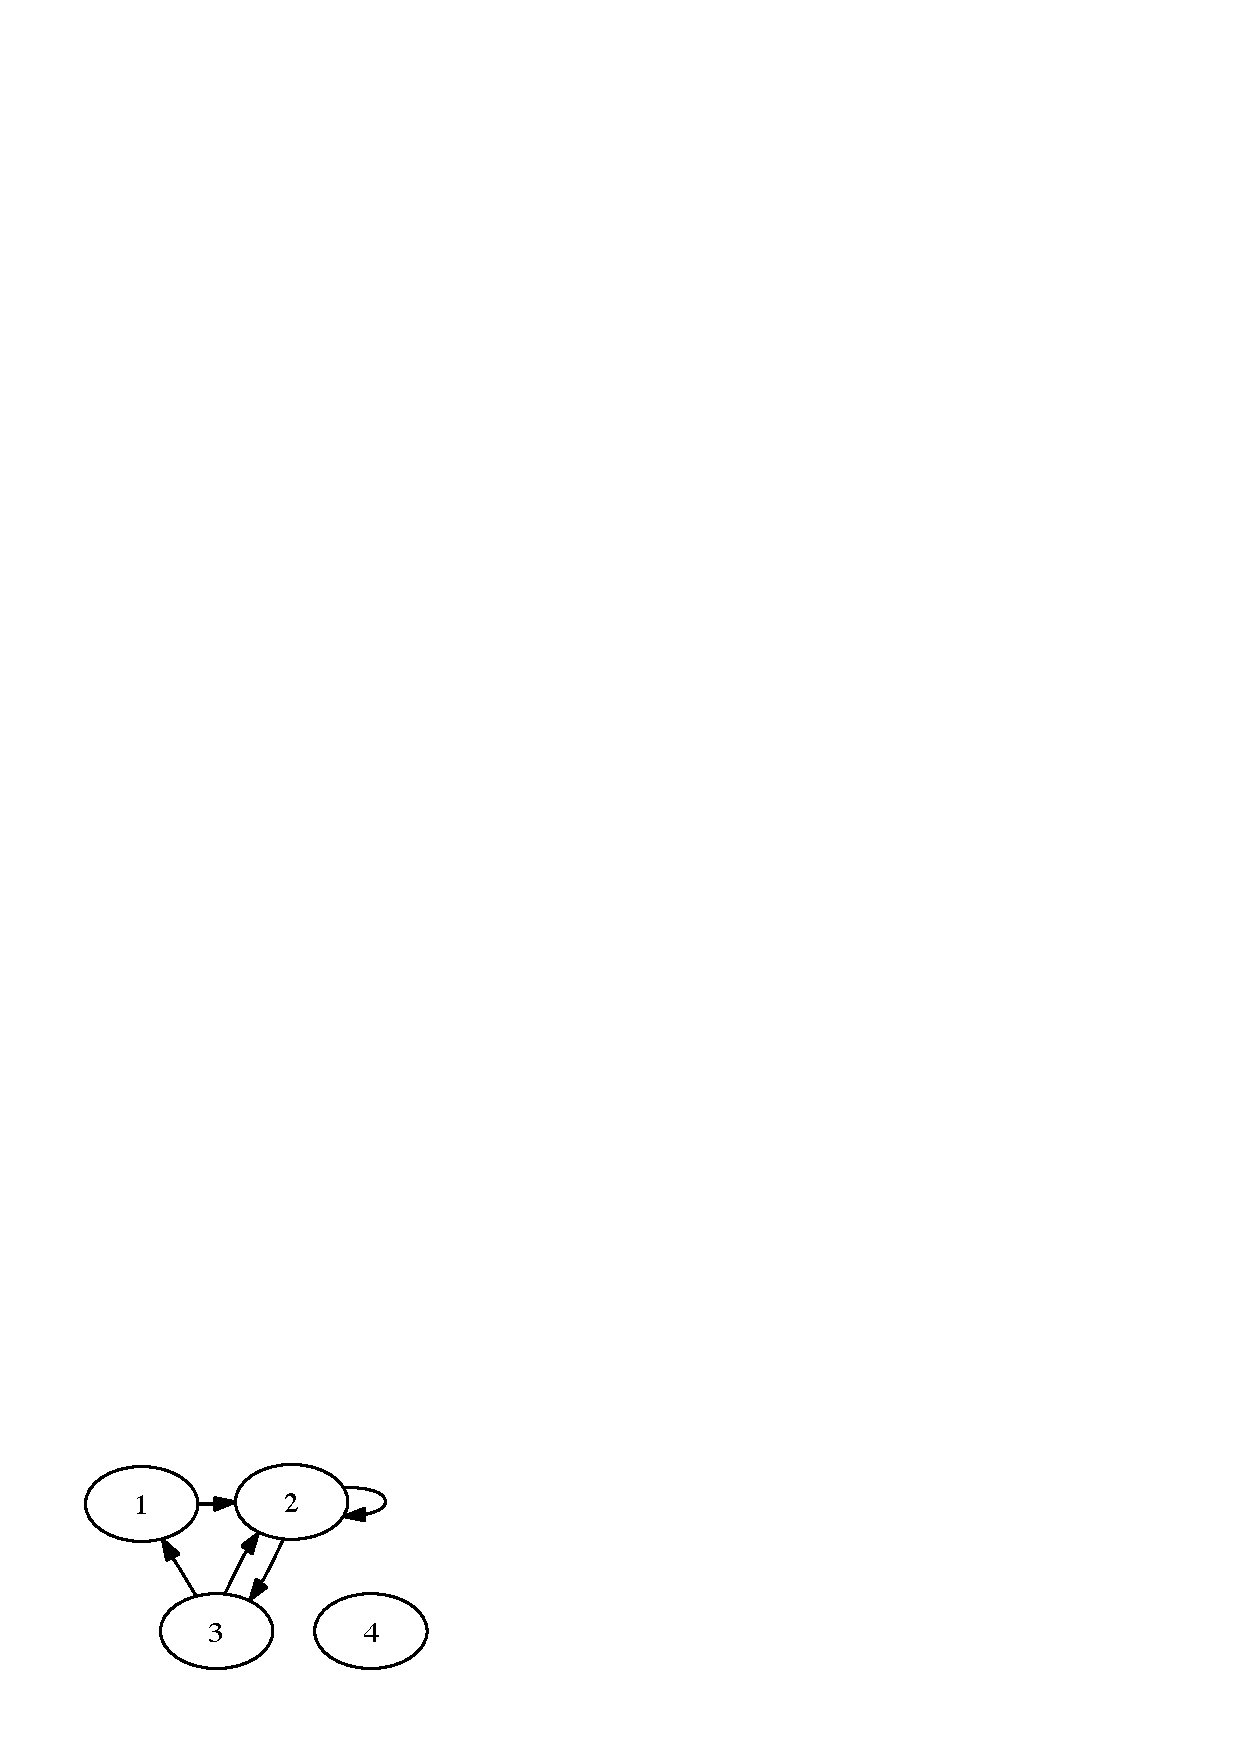
\includegraphics[width=0.3\textwidth]{digraph}
  \caption{A finite directed graph $G$}
  \label{fig:digraph}
\end{figure}
%
One common representation of such graphs uses a pair of lists
$(\ell_V, \ell_A)$, where $\ell_V$ is the list of vertex labels and
$\ell_A$ is the \emph{adjacency list} representing the arrows by
pairing the labels of each source and target. For the above graph $G$,
$\ell_V = [1, 2, 3, 4]$ and $\ell_A = [(1,2), (2,2), (2,3), (3,2),
(3,1)]$.
%
Thus we define the datatype of graphs as\footnote{We use Haskell
  notation in which $[t]$ is the type of lists of elements of
  type~$t$, and $(t_1, t_2)$ is the cartesian product of types~$t_1$
  and~$t_2$.}
%
\begin{lstlisting}[language=Haskell]
type Graph = ([Int], [(Int, Int)])
\end{lstlisting}
%
However, this is not a complete description of the intended
representation, as there are representation invariants and conditions
not expressed by the type, e.g.,
%
\begin{enumerate}
\item The order in which vertices and arrows are listed is not
  important%
; for example, $[1,2,3,4]$ and $[4,1,2,3]$ represent the same vertices.
\item Each vertex and arrow must be listed exactly once.
\item The source and target of each arrow must appear in the list of vertices.
\end{enumerate}
%
Thus, to implement the mathematical set~$\mathsf{Graphs}$, we must not
only decide on the underlying datatype $\mathtt{graph}$, but also
determine what values of that type represent which elements
of~$\mathsf{Graphs}$. All this can be expressed with a \emph{realizability
  relation}
%
\begin{equation*}
  r \rz x
\end{equation*}
%
which is read as ``$r$ realizes $x$''. In the above example we would
write
%
\begin{equation*}
([1, 2, 3, 4], [(1,2), (2,2), (2,3), (3,2), (3,1)]) \rz G.
\end{equation*}
%
We now give a precise definition.


\begin{definition}[Assemblies]
  Let $A$ be a TPCA and $\comp{A}$ a sub-TPCA. An \emph{assembly}
  over~$(A, \comp{A})$ is a triple $(S, |S|, {\rz_S})$ where $S$ is a
  set, $|S|$ is a type, and $\rz_S$ is a relation between $A_{|S|}$
  and~$S$ satisfying: for every $x \in S$ there is $r \in A_{|S|}$
  such that $r \rz_S x$.

  A \emph{realized map} $f : S \to T$ between assemblies $(S, |S|,
  {\rz_S})$ and $(T, |T|, {\rz_T})$ is a map for which there exists $p
  \in \comp{A}_{|S| \to |T|}$ satisfying: if $r \rz_S x$ then $\defined{p
    \cdot r}$ and $p \cdot r \rz_T f(x)$.

  Assemblies and realized maps form the \emph{category
    $\Asm{A,\comp{A}}$ of assemblies over $(A, \comp{A})$}.
\end{definition}

\noindent
There are many versions of realizability. Ours is known as \emph{typed
  relative realizability}. It is typed because we used typed PCAs
rather than the ordinary ones. It is relative because we used one
TPCA~$A$ for assemblies, and another for the realized maps. By this we
are capturing the idea that computable functions may operate on
potentially non-computable data, as was the case for type~2 machines
and the graph model, cf.\ Sections~\ref{sec:type-2}
and~\ref{sec:graph-model}. In the typical case the larger TPCA~$A$
allows representation of arbitrary data, but the sub-TPCA $\comp{A}$
consists only of the computable part of~$A$ which forces the realizers
for maps to be computable. Thus it makes sense to say in the general
case that the maps are realized \emph{relative} to the choice of a
sub-TPCA~$\comp{A}$.

When $A$ is not typed the definition of an assembly simplifies a bit
because we need not keep mentioning the (trivial) types: an assembly
over a PCA~$A$ is a pair $(S, {\rz_S})$ where $S$ is a set and $\rz_S$
is a relation between~$A$ and~$S$, such that for every $x \in S$ there
is $r \in A$ and $r \rz_S x$.

Another special case occurs when $\comp{A} = A$. In this case we write
$\Asm{A}$ instead of $\Asm{A,A}$.

Normally the TPCA $A$ will actually be an NR-TPCA, and $\comp{A}$ a
sub-NR-TPCA of~$A$.

Particular choices of a TPCA with sub-TPCA yield well known ``schools
of computable mathematics'':
%
\begin{enumerate}
\item When $A = \comp{A} = \NN$ is the first Kleene algebra we get the
  Russian school of \emph{recursive
    mathematics}~\cite{recursive-math}, also known as \emph{type I
    computability} because the underlying computational model is that
  of type~1 machines.
\item When $A = \Baire$ is the second Kleene algebra we get Kleene's
  \emph{function realizability}~\cite{KleeneSC:fouim}, also known by
  its newer name \emph{type two effectivity (TTE)}~\cite{tte}. There
  are actually three variants:
  %
  \begin{enumerate}
  \item $A = \comp{A} = \Baire$ is \emph{continuous} function
    realizability because maps are realized by arbitrary continuous
    realizers,
  \item $A = \Baire$ and $\comp{A} = \comp{\Baire}$, where
    $\comp{\Baire}$ is the set of computable sequences, is the
    \emph{relative} type 2 realizability,
  \item $A = \comp{A} = \comp{\Baire}$ is the \emph{computable}
    function realizability.
  \end{enumerate}
  %
  We will mostly study the continuous and the relative function
  realizaiblity.
\item When $A = \Scott$ is the graph model we get a version of
  realizability that is closely related to equilogical
  spaces~\cite{BauerA:equs}. Here two there are three variants:
  %
  \begin{enumerate}
  \item $A = \comp{A} = \Scott$ is the continuous model,
  \item $A = \Scott$ and $A = \comp{\Scott}$ is the family of
    c.e.~sets is the relative model,
  \item $A = \Scott = \comp{\Scott}$ is the computable model.
  \end{enumerate}
\item Closely related to the previous case is $A = U$ where~$U$ is a
  universal Scott domain~\cite{GunterScott}. This again gives as three
  variants of \emph{domain representations}~\cite{Bla97,Bla97a}.
\item The case $A = \PCFinf$ and $\comp{A} = \PCF$, cf.
  Section~\ref{sec:pcf} is interesting because we may actually test
  the performance of PCF realizers by running them as Haskell
  programs.
\end{enumerate}
%
In Section~\ref{variants} we shall study some of these in greater
detail.




\section{Equivalent formulations}
\label{sec:representations-formulations}

\subsection{Assemblies and modest sets}
\label{sec:assemblies}

\subsection{Partial equivalence relations}
\label{sec:pers}

\subsection{Representations}
\label{sec:representations}


\section{Type 1 representations}
\label{sec:type-1-representations}

\section{Type 2 representations}
\label{sec:tte-representations}

Admissibility.

\section{Equilogical spaces and domain representations}
\label{sec:equilogical-spaces}

\section{A convenient category of spaces}
\label{sec:qcb-spaces}



%%% Local Variables: 
%%% mode: latex
%%% TeX-master: "notes"
%%% End: 
 % Week 3, 4, 5
\chapter{The Internal Language}
\label{chap:internal-language}

\section{Constructions of assemblies}
\label{sec:constructions}

\subsection{Products and equalizers}
\label{sec:products-equalizers}

% terminal object

\subsection{Coproducts and quotients}
\label{sec:products-equalizers}

% initial object

\subsection{Epis and monos}
\label{sec:epis-monos}

% When is a numbered set total

\subsection{Factorization of morphisms}
\label{sec:factorization}

% Explicitly state regularity

\subsection{Cartesian closed structure}
\label{sec:ccc}

\subsection{Families of assemblies}
\label{sec:dependent-types}

% Uniform families

% Dependent products and sums

% State lccc

\subsection{Projective assemblies}
\label{sec:projective-assemblies}

% Presentation axiom

\begin{definition}
  An assembly is \emph{canonically projective} if each element has
  precisely one realizer.
\end{definition}

\noindent
In symbols, an assembly $S$ is canonically projective when, for all
$x, y \in S$, $r \in A_{|S|}$,
%
\begin{equation*}
  r \rz_S x \land r \rz_S y \implies x = y.
\end{equation*}
%
The canonically projective assemblies are, up to isomorphism,
precisely the projective objects of the category of assemblies.

A canonically projective modest set $(S, |S|, {\rz_S})$ is determined,
up to isomorphism, by the set of the total realizers~$\|S\|$. This
follows from Lemma~\ref{lemma:iso-assembly} and the fact that
projectivity ensures that $S$ and $\|S\|$ are in bijective
correspondence. This combined with the fact that every modest set is a
quotient of a canonically projective one leads to the following
definition.

Let $\subcat{A, \comp{A}}$ be the category whose objects are pairs
$(S, |S|)$ where $|S|$ is a type and $S \subseteq A_{|S|}$. A morphism
$f : (S, |S|) \to (T, |T|)$ is a map $f : S \to T$ which is tracked by
some $p \in \comp{A}_{|S| \to |T|}$, i.e., for all $p \in S$,
$\defined{p\,r}$ and $p\,r \in T$. This category is equivalent to the
full subcategory of $\Mod{A, \comp{A}}$ on the canonically projective
modest sets.


\section{The realizability interpretation of logic}
\label{sec:realizability-interpretation}

\section{Realizability toposes}
\label{sec:realizability-toposes}

\section{From constructive to computable mathematics}
\label{sec:constructive-math}



%%% Local Variables: 
%%% mode: latex
%%% TeX-master: "notes"
%%% End: 
 % Week 6, 7
\chapter{Computable Mathematics}
\label{chap:computable-mathematics}

\section{Natural numbers}
\label{sec:natural-numbers}

% Definition

% Countable assemblies

\section{Inductive and coinductive spaces}
\label{sec:inductive-coinductive}


\section{Real numbers}
\label{sec:real-numbers}

\section{Metric spaces}
\label{sec:metric-spaces}


\section{Function spaces}
\label{sec:function-spaces}

\subsection{Are all functions continous?}
\label{sec:all-fun-cont}

\subsection{Multi-valued functions}
\label{sec:multi-valued-functions}



\section{Hyperspaces}
\label{sec:hyperspaces}


\section{Functionals}
\label{sec:functionals}


\section{Topological spaces}
\label{sec:topological-spaces}



%%% Local Variables: 
%%% mode: latex
%%% TeX-master: "notes-on-realizability"
%%% End: 
 % Week 8, 9, 10, 11, 12, 13

\chapter{Implementation}
\label{chap:implementation}


%%% Local Variables: 
%%% mode: latex
%%% TeX-master: "notes"
%%% End: 
    % Week 14, 15



%%%%%%%%%%%%%%%%%%%%%%%%%%%%%%%%%%%%%%%%%%%%%%%%%%%%%%%%%%%%%%%%%%%%%%
%%%% Bibliography

\clearemptydoublepage

\bibliographystyle{plain}
\addcontentsline{toc}{chapter}{\numberline{}Bibliography}
\markboth{}{Bibliography}

{
\renewcommand{\markboth}[2]{}
\bibliography{realizability,cca,notes}
}

%%%%%%%%%%%%%%%%%%%%%%%%%%%%%%%%%%%%%%%%%%%%%%%%%%
% INDEX
% \clearemptydoublepage

% \addcontentsline{toc}{chapter}{\numberline{}Index}

% \markboth{}{Index}

% {
% \renewcommand{\markboth}[2]{}
% \printindex
% }


\end{document}
